\documentclass[12pt,twoside]{article}

\usepackage[T1]{fontenc}
\usepackage[utf8]{inputenc}
\usepackage[spanish]{babel}

\let\layoutspanish\relax
\addto\captionsspanish{\def\tablename{Tabla}}
\unaccentedoperators

\usepackage[a4paper]{geometry}
  \geometry{hmargin={2.5cm,2.5cm},height=22cm}
  
\renewcommand{\baselinestretch}{1.2}  
\setlength{\partopsep}{0pt}
\setlength{\itemsep}{0pt}
\setlength{\topsep}{0pt}
\setlength{\parsep}{0pt}
\setlength{\parskip}{0.25\baselineskip}

\renewcommand{\textfraction}{0.1}
\renewcommand{\topfraction}{1}
\renewcommand{\bottomfraction}{1}
\renewcommand{\floatpagefraction}{1}

\setcounter{totalnumber}{5}
\setcounter{topnumber}{3}
\setcounter{bottomnumber}{2}

\usepackage{caption}
\setcaptionwidth{\textwidth}
\addtolength{\captionwidth}{-2\parindent}
\captionsetup{margin=\leftmargini,%
  width=\captionwidth,%
  labelfont={up,bf},%
  font={small,sl},%
  %indention={\captionindent
}

\usepackage{indentfirst}

\usepackage[pdftex]{color}

\usepackage[pdftex]{graphicx}

\usepackage{amsmath}
\allowdisplaybreaks 
\usepackage{amssymb}
\usepackage{amsfonts} 
\usepackage{enumerate}

\usepackage{fancyhdr}

\newcommand{\RunningAuthor}{Ginés Meca Carbonell}
\newcommand{\Author}[1]{\renewcommand{\RunningAuthor}{#1}}
\renewcommand{\leftmark}{\RunningAuthor}

\newcommand{\RunningTitle}{Métodos de Machine Learning basados en Árboles de Decisión.}
\newcommand{\Title}[1]{\renewcommand{\RunningTitle}{#1}}
\renewcommand{\rightmark}{\RunningTitle}

\pagestyle{fancy}
\fancyhf{}
\fancyhead[LO]{\small \slshape \leftmark}    
\fancyhead[RE]{\small \slshape \rightmark}   
\fancyhead[RO,LE]{\small \slshape \thepage}  

\renewcommand{\headrulewidth}{0.6pt}         
\renewcommand{\footrulewidth}{0pt}           
                                             
\setlength{\headheight}{1.5\headheight}      

\fancypagestyle{plain}{%                     
  \fancyhf{}                                 
  \setlength{\headwidth}{\textwidth}
  \fancyfoot[C]{\small \slshape \thepage}    
  \renewcommand{\headrulewidth}{0pt}
  \renewcommand{\footrulewidth}{0pt}
  }
  
\newcommand{\abs}[1]{\ensuremath{|#1|}}

\usepackage{hyperref}

\title{Métodos de Machine Learning basados en Árboles de Decisión}
\author{Ginés Meca Carbonell\\*[1em]
\begin{minipage}{0.75\textwidth}
\footnotesize \itshape
\begin{center}
Universidad de Alicante \\
4º de Grado en Matemáticas
\end{center}
\end{minipage}
}
\date{Junio 2022}

\usepackage{pdfpages}




\begin{document}


\includepdf[pages=1]{anexo-1-portada-memoria-tfg-matematicas.pdf}



\section*{Resumen}

\emph{En este trabajo, se ha estudiado el conjunto de algoritmos de Machine Learning derivados de los árboles de decisión.}

\newpage



\section*{Abstract}

\emph{}

\newpage



\tableofcontents



\newpage



\section{Introducción}

Vivimos en la era de la información. Cada segundo, millones de datos viajan entre diferentes lugares del planeta y se guardan formando enormes conjuntos de datos. Además, cada vez hay más instrumentos capaces de recoger información. Donde antes se necesitaba hacer uso de encuestas, ahora nos encontramos con dispositivos, como los teléfonos móviles, capaces de escribir texto, recoger audio y realizar fotografías y vídeos. Así, la información a nuestra alcance es infinita. Podemos conocer cuáles son los conceptos que son tendencia en los buscadores de internet, o cuáles son aquellos audiovisuales que más éxito están teniendo en las redes sociales. Del mismo modo, podemos acceder al historial de imágenes de la cámara de seguridad de nuestra vivienda o a la tabla que recoge las últimas operaciones de nuestra empresa. Es fácil obtener grandes cantidades de datos de aquello que nos interesa.

Dado que el número de datos que manipulamos cada vez es mayor,las técnicas utilizadas para analizarlos van evolucionando constantemente. Muchas de las técnicas clásicas del análisis de datos han quedado obsoletas, otras se utilizan para crear algoritmos más complejos. En este trabajo, trataré de abordar todos aquellos algoritmos derivados de los árboles de decisión.

Dado que en los últimos años varios alumnos han realizado su TFG sobre árboles de decisión explicando su estructura más básica, resumiré las secciones dedicadas a ello con el fin de centrarme en analizar a fondo los algoritmos más complejos y novedosos que no se han tratado en estos trabajos y, así, elaborar un mapa conceptual de modelos.



\subsection{Datos: Llueve en Australia}

Para hacernos una idea de cómo funciona cada uno de los algoritmos detallados a lo largo del trabajo, haremos uso del conjunto de datos indicado. Se trata de un dataset en el que podemos encontrar mediciones de diferentes variables meteorológicas así como la fecha y localidad correspondientes y la información relativa a si llovió o no el día de la medición y el día siguiente.

\begin{figure}[h]
	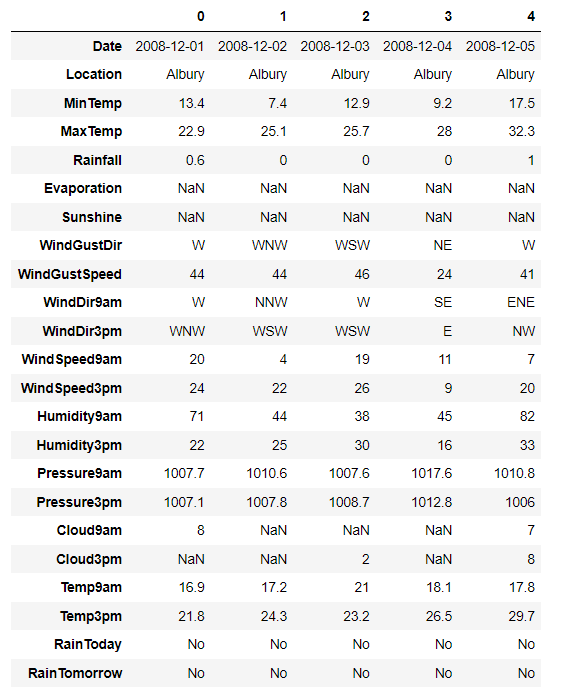
\includegraphics[width = \textwidth]{Intro_01}
	\caption{Encabezado del dataset}
\end{figure}

En total, se tiene 23 columnas que recogen información de 145460 días.


\subsection{Metodología}

A la hora de aplicar los diferentes métodos al conjunto de datos se procederá mediante validación cruzada. Es decir:

\begin{enumerate}
\item Se selecciona el modelo correspondiente.
\item Se separa, al azar, el conjunto de datos inicial en dos: datos de entrenamiento y datos de testeo.
\item Se entrena el modelo con los datos de entrenamiento.
\item Se aplica el modelo entrenado a los datos de testeo.
\item Se comprueba la veracidad de las predicciones realizadas.
\end{enumerate}

Además, los cálculos se realizarán en el lenguaje de programación Python. Todo el código se encuentra disponible en el Anexo (\ref{sec:Anexo}).



\newpage



\section{Árboles de decisión CART}
\subsection{Preliminares}

Los árboles de decisión son muy utilizados como método predictor (tanto de regresión como de clasificación) dada si simpleza, su efectividad y lo visual que resulta su funcionamiento a través de un gráfico, lo cual facilita su comprensión. Se trata de un algoritmo que divide sucesivamente el conjunto inicial de datos en diferentes subconjuntos a través de diversas condiciones relacionadas con sus variables explicativas. Por ejemplo:

\textbf{Ejemplo 1: } \textit{Se pretende estudiar la variable 'RainTomorrow' del conjunto de datos dado en función de las variables explicativas 'Cloud3pm' y 'Humidity3pm'(nivel de nubosidad y de humedad a las 15.00, respectivamente) para predecir si lloverá o no al día siguiente. Así, escogiendo únicamente las variables explicativas indicadas, el esquema que seguirá nuestro árbol de clasificación será el siguiente: }
\begin{figure}[h]
	\centering
	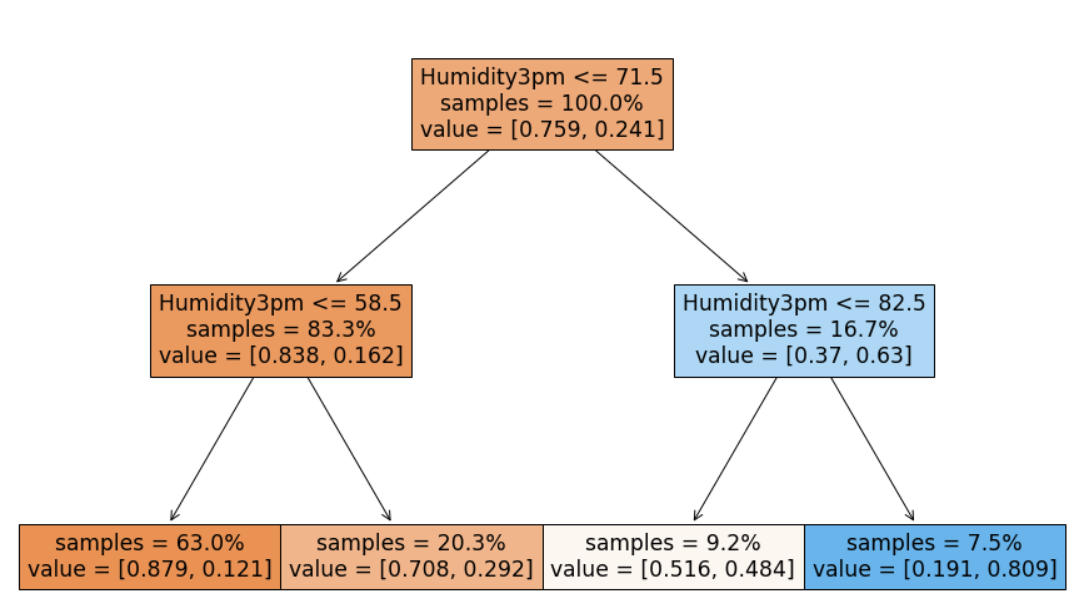
\includegraphics[width = 0.7\textwidth]{ex2_1_01}
	\caption{Ejemplo 2.1. Árbol de decisión}
	\label{fig:Ejemplo 1}
\end{figure}

Como se puede observar, el algoritmo es muy intuitivo: se introduce un individuo y se le aplica la primera condición; si la respuesta es afirmativa se sigue el camino de la izquierda y si es negativa el de la derecha. Mediante este proceso, se van comprobando si sus variables explicativas cumplen las diferentes condiciones que se planteen hasta llegar a un grupo que deja de dividirse que será su predicción.

Por otro lado, es fácil ver que las condiciones del algoritmo se corresponden con una partición del espacio. Como en el ejemplo anterior se han elegido únicamente dos variables explicativas, se puede hacer una representación de los individuos sobre $\mathbb{R}^{2}$ y determinar sobre él las diferentes regiones de predicción.
\begin{figure}[h]
	\centering
	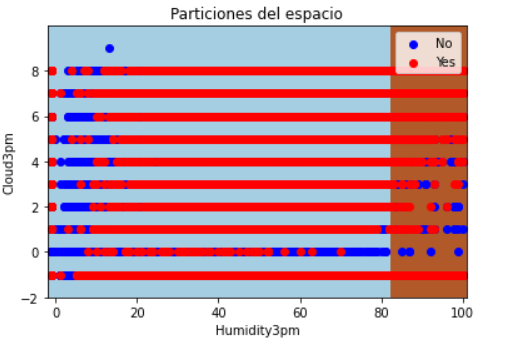
\includegraphics[width = 0.5\textwidth]{ex2_1_02}
	\caption{Partición del espacio del Ejemplo 2.1}
	\label{fig:Ejemplo 2.1.2}
\end{figure}


\subsubsection{Notación y conceptos básicos}

A continuación, se introducirán una serie de términos básicos para poder hacer referencias correctas a los conceptos presentados. Por un lado, nos encontramos con las siguientes definiciones:
\begin{description}
\item[Nodo raíz: ]Primer nodo, que contiene a todos los individuos, a partir del cual comienzan a realizarse las divisiones.
\item[Nodo interno: ]Nodos intermedios que provienen de una división y desencadenan otra. Dentro de ellos, se pueden definir:
	\begin{description}
	\item[Nodo padre: ]Nodo anterior al nodo interno que hemos fijado.
	\item[Nodos hijos: ]Nodos resultantes de la división del nodo interno fijado.
	\end{description}
\item[Nodo hoja: ]Nodos finales que dan lugar a la predicción.
\end{description}

Se pueden identificar todos estos nodos en la figura del ejemplo 1 (\ref{fig:Ejemplo 2.1}). Se tienen un nodo raíz, seis nodos internos y 8 nodos hoja.

Por otro lado, conviene hablar del concepto de sobreajuste (en inglés: overfitting). Se dice que un modelo se encuentra sobreajustado si el algoritmo se ha adaptado en exceso a los individuos del conjunto de entrenamiento del mismo. Este hecho provoca que la predicción de los individuos de este conjunto sea muy buena, mientras que al introducir nuevos individuos estas predicciones presentan grandes errores.

Para lidiar con el sobreajuste, interesa manejar también otras dos nociones: el sesgo y la varianza. El sesgo (en inglés: bias) hace referencia a los errores cometidos en las predicciones de los individuos de nuestro conjunto de entrenamiento. Por contra, la varianza es la medida del error cometido en los individuos que no pertenecen a este conjunto; en nuestro caso, lo mediremos en los individuos del conjunto de testeo. No obstante, estos conceptos generan un problema: interesa tener valores bajos de ambos indicadores, pero disminuir el sesgo conlleva un aumento de la varianza. Así, a la hora de construir un modelo de Machine Learning, interesa estudiar que el sesgo no sea excesivamente bajo, para evitar el sobreajuste, pero también que no sea excesivamente alto para que las predicciones sean fiables.


\subsubsection{Objetos de estudio de un CART}

Una vez visto cómo se realizan las predicciones al trabajar con árboles de decisión, corresponde explicar el funcionamiento del mismo. Para ello, habrá que tratar los siguientes aspectos:
\begin{enumerate}
\item Elección de variables y valores asociados a cada nodo interno.
\item Criterio de parada de división de los nodos
\item Valor o clase asignada a cada nodo
\end{enumerate}


\subsection{Elección de variables y valores asociados a cada nodo interno} \label{sec: subsec22}
Sea un conjunto de datos de n individuos y p+1 variables ($n,p \in \mathbb{N}$). De este modo, sean $X_1, X_2, ... , X_p$ las variables explicativas e $y$ la variable dependiente. En el caso de nuestro conjunto de datos de ejemplo:
\begin{table}[h]
\centering
\begin{tabular}{rcccc|c}
 & \multicolumn{1}{l}{$X_1$}         & $X_2$                        & ...                      & $X_{22}$ & $y$ \\ \hline
\multicolumn{1}{l|}{$x_1$} & \multicolumn{1}{r|}{2008-12-01} & \multicolumn{1}{l|}{Albury} & \multicolumn{1}{l|}{...} & No        & \multicolumn{1}{l|}{No} \\ \hline
\multicolumn{1}{l|}{$x_2$} & \multicolumn{1}{r|}{2008-12-02} & \multicolumn{1}{l|}{Albury} & \multicolumn{1}{l|}{...} & No        & \multicolumn{1}{l|}{No} \\ \hline
\multicolumn{1}{l|}{$x_3$} & \multicolumn{1}{r|}{2008-12-03} & \multicolumn{1}{l|}{Albury} & \multicolumn{1}{l|}{...} & No        & \multicolumn{1}{l|}{No} \\ \hline
\end{tabular}
\end{table}

Pese a las similitudes existentes entre los árboles de regresión y los de clasificación, conviene dividir este apartado en dos con tal de mostrar el funcionamiento exacto de cada uno de ellos.


\subsubsection{Árboles de regresión}
Se busca conocer cómo realizar las divisiones. En particular, nos centraremos en la primera división y el proceso será similar para las siguientes. Al situarnos en el nodo raíz, nos encontramos con el conjunto de datos al completo y pretendemos dividirlo en dos regiones, que denotaremos $R_1$ y $R_2$, en función de una de las variables explicativas, $X_j$, y de un valor respecto de esta, s, de manera que:
\begin{equation*}
R_1 (j,s) = \{ X | X_j \leq s \} \, \, \, \wedge \, \, \,  R_2 (j,s) = \{ X | X_j > s\}
\end{equation*}

Sabemos que $Y_1$ se mantendrá constante sobre $R_1$ y que $Y_2$ también será constante sobre $R_2$. De esta manera, buscamos j y s tales que:
\begin{equation*}
\min_{j,s}(\min_{c_1, c_2}(\sum_{x_i \in R_1}(y_i - c_1)^2 + \sum_{x_i \in R_2}(y_i - c_2)^2))
\end{equation*}
o lo que es lo mismo, buscamos j y s que minimicen el error cometido en la predicción de los individuos del conjunto de entrenamiento. Esta tarea se puede llevar a cabo probando todos los casos posibles y escogiendo el que minimice la expresión.


\subsubsection{Árboles de clasificación}
En el caso de los árboles de clasificación, la variable dependiente es una clase; es decir, como en la tabla dada al comienzo de la subsección (\ref{sec: subsec22}). Ahora, en lugar del error mínimo cuadrático, introduciremos una función de impureza que nos permita evaluar la homogeneidad de los nodos; es decir, que nos permita estudiar qué acciones separan mejor el espacio en función de las diferentes clases.


\subsection{Criterio de parada de escisión de nodos}
Se podría pensar que la precisión de un CART aumenta conforme aumenta en profundidad, es decir, conforme aumenta en número de particiones. No obstante, como ya se ha introducido, cuantas más particiones del espacio realice el algoritmo, más se estará ajustando a los datos del conjunto de entrenamiento, lo que puede llevar a sobreajuste. Con tal de evitar este hecho, se han implementado algunos métodos de "poda" del árbol. Es evidente que podando el árbol se introduce sesgo, pues no dejamos que se adecue totalmente a los datos de entrenamiento; sin embargo, haciendo esto de manera controlada se consigue disminuir la varianza y mejorar las predicciones.

Por un lado, la técnica más simple consiste en establecer una profundidad máxima. Con esta condición, se puede asegurar que los nodos dejarán de dividirse una vez alcanzado el nivel indicado. Por ejemplo, en el Ejemplo 2.1 (Figura \ref{fig:Ejemplo 2.1}) se ha establecido una profundidad máxima igual a 3.

Por otro lado,


\subsection{Valor o clase asignada a cada nodo hoja}
Como se comentaba anteriormente, el resultado de un árbol de decisión es una partición del espacio. Supongamos que se obtienen M regiones diferentes denotadas por $R_{m}$ con $m = 1, ..., M$. Por tanto, definamos como Y al árbol de decisión y como $c_m$, con $m = 1,...,M$, a las predicciones (imágenes de Y) asociadas a cada región $R_m$. De este modo:
\begin{equation*}
Y(x) = \sum^M_{m = 1} c_{m}I(x \in R_m) \, \, \, \forall x \in D
\end{equation*}
donde D es el dominio de la función (espacio de las variables explicativas) e I es la función indicadora:
\begin{equation*}
I(x) = 
\left.
\begin{array}{ccc}
1 & si & x \in R_m \\
0 & si & x \not\in R_m 
\end{array}
\right\}
\end{equation*}


Así, a la hora de entrenar un modelo, se busca minimizar los errores entre y e Y. Por ejemplo, si tomamos el error mínimo cuadrático, llegamos al problema:
\begin{equation*}
\min_{Y_i} \sum_{i=1}^n (y_i - Y_i)^2 \Rightarrow \min_{c_m} \sum_{m = 1}^M \sum_{x_i \in R_m} (y_i - c_m)^2
\end{equation*}
donde $Y_i = Y(x_i) \, \, \forall i=1,...n$. Si denotamos $f(c_m) = \sum_{x_i \in R_m} (y_i - c_m)^2$, observamos que alcanzar la solución óptima del problema planteado es equivalente a minimizar la función f:
\begin{equation*}
f'(c_m) = -2 \sum_{x_i \in R_m} (y_i - c_m) = -2 \sum_{x_i \in R_m}y_i + 2n_mc_m = 0 \Leftrightarrow c_m = \frac{1}{n_m} \sum_{x_i \in R_m}y_i
\end{equation*}
donde $n_m$ es el conjunto de datos pertenecientes a la región $R_m$, $\forall m = 1,...M$.

En conclusión, el valor asignado a cada nodo hoja será la media de las observaciones de los individuos del conjunto de entrenamiento que pertenecen a dicho nodo.


\subsection{Ejemplo}



\subsection{Ventajas y desventajas}





\section{Anexo} \label{sec:Anexo}
Todo el código empleado en la elaboración de los ejemplos se encuentra en la carpeta de GitHub creada para tal fin (\url{link})
\end{document}